(code/code03.ijm)

The above operation concatenates content of \ilcom{text2} to the content of \ilcom{text1} and produces a third variable \ilcom{text3} that holds the result of concatenation. It should be noted here, that macro has two ways of usage for \ilcom{+}. What we tested in above is ``concatenation''. Another usage is ``addition'' in the next section.

\begin{indentexercise}
{1}
\item Add more string variables and make a longer sentence.\\

\item **Answer**: One example could be as shown in the figure \ref{var_stringconcat}. 
\begin{figure}[htbp]
\begin{center}
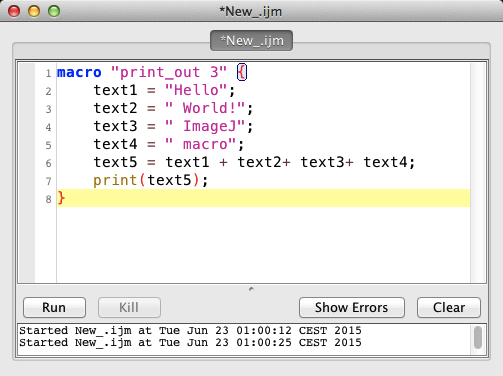
\includegraphics[scale=0.6]{fig/var_stringContcat.png}
\caption{Concatenating many strings} \label{var_stringconcat}
\end{center}
\end{figure}

\end{indentexercise}

It is also possible to store a number in a variable. For example, \\